\documentclass[
	aps, pra,
	superscriptaddress, twocolumn,
	floatfix,
	10pt
]{revtex4-1}

\usepackage{silence}
\WarningFilter{revtex4-1}{Repair the float}  % to remove annoying revtex message
\usepackage[final]{graphicx}
\graphicspath{{./figures/}}
\usepackage{times,bbm,amsmath,amssymb}
\usepackage{microtype}
\usepackage{epsfig,color}
\usepackage[dvipsnames]{xcolor}
\usepackage{hyperref}
\hypersetup{
    colorlinks = true
}
\usepackage{cleveref}

\usepackage{libertine}

\usepackage{float,siunitx}
\usepackage[caption = false]{subfig}

% \usepackage[english]{babel}
% \usepackage{thumbpdf,enumerate}
\usepackage{booktabs}
% \usepackage{sidecap}
% \usepackage[scaled=.8]{couriers}    
% \usepackage{pstricks}
\usepackage{multirow}
\usepackage{placeins}
\usepackage{relsize}  
% \usepackage{pst-grad,bm}
% \usepackage{epigraph}
\usepackage{gensymb}  % for the \degree command
% \usepackage{longtable}
% \usepackage{booktabs}

% \usepackage{soul}
% \usepackage{ulem}
% \normalem 

\usepackage{acronym}
% \usepackage{todonotes}
\usepackage{easyReview}

\usepackage{tikz}
\usetikzlibrary{quantikz}
\usepackage{physics}

\newcommand{\bs}[1]{\boldsymbol{#1}}
\newcommand{\on}[1]{\operatorname{#1}}
\newcommand{\parTitle}[1]{\noindent{\color{Mahogany}(\emph{#1})}}

\newcommand{\CC}{\mathbb{C}}
\newcommand{\PP}{\mathbb{P}}
\newcommand{\RR}{\mathbb{R}}
\newcommand{\ZZ}{\mathbb{Z}}

\newcommand{\calC}{{\mathcal{C}}}
\newcommand{\calE}{{\mathcal{E}}}
\newcommand{\calH}{{\mathcal{H}}}
\newcommand{\calS}{{\mathcal{S}}}
\newcommand{\calP}{{\mathcal{P}}}
\newcommand{\calO}{{\mathcal{O}}}
\newcommand{\calU}{{\mathcal{U}}}
\newcommand{\calV}{{\mathcal{V}}}
\newcommand{\calW}{{\mathcal{W}}}
\newcommand{\MP}[1]{\textcolor{blue}{Mauro: #1}}


\begin{document}
\title{Entanglement transfer and retrieval via quantum-walk-based qubit-qudit dynamics}
%\title{Quantum walks with entangled qubits: notes for Rome} 
\author{Belfast, August 2019}

\begin{abstract}
Entanglement is a key feature of quantum mechanics that results in a fundamental resource for quantum information tasks, such as quantum cryptography, communication and computation. Furthermore this capability to enhance security and computational power is straightened by the use of high-dimension entangled states. However the generation and the control of such high-dimensional quantum correlations makes the problem  challenging with the current quantum technologies.  Here we propose a quantum walk-based protocol to accumulate and transfer entanglement between Hilbert spaces with dimension greater than two. In particular, we illustrate a possible implementation in a photonic platform in which the information is encoded in the angular momentum degree of freedom. The choice of investigating quantum walks is motivated by their generality and versatility in implementation in several physical systems. Hence, given the cross-cutting role of quantum walks in quantum information, our protocol can represent  a  powerful and general tool for controlling entanglement generation in high-dimension.
\end{abstract}
\maketitle


\section{Introduction}
\parTitle{Interfacing systems of different dimensionality}
The interface between quantum systems of different dimensionality offers a rich venue of investigation at both the fundamental and technological level. On one hand, the relation between correlations and the dimension of a quantum system becomes particularly relevant when considering parties living in Hilbert spaces of different dimensions. 
%An extreme instance is that of a compound consisting of a  system with infinite-dimensional state space and a discrete system with finite D-dimensional Hilbert space. 
On the other hand, promising architectures for quantum communication, such as quantum repeaters~\cite{Lvovsky2009}, rely on interfaces between hetero-dimensional systems such as light and matter-like systems, and their efficient implementation is based on the availability of such technological tools~\cite{Kimble2008,Hammerer2010,Brask2010}.

\parTitle{What is a good interface?}
A reliable interface should connect systems of different dimensionalities in order to transfer key quantum resources, thus enabling the implementation of quantum information protocols.
% while being faithful to their inherent structure.
In this context, being able to transfer a key quantum resource such as entanglement is paramount.
This would allow to establish long-haul quantum channels in delocalized architectures for quantum communication~\cite{Kimble2008} and distributed quantum computing~\cite{Collins2001,Eisert2000,Huelga2001,Huelga2002,Paternostro2003}. Moreover, by arranging special forms of entangled states in systems of low dimension (and thus easily controllable), an interface designed for effective entanglement transfer could be used to siphon quantum correlation into high-dimensional information carriers, whose reliable preparation is otherwise notoriously demanding.
Proposals for interfaces between a continuous-variable and a two-dimensional system have been put forward in a number of physical settings, ranging from cavity- and circuit-quantum electrodynamics to polar molecules close to superconducting resonators or quantum dots and color-centers in diamonds in defect-microcavities and photonic crystals \highlight{(references)}. 

\parTitle{Recent experimental advances}
Recent experimental advances in the management of finite high-dimensional quantum systems enabled by the growing capacity to prepare, manipulate and measure the orbital angular momentum (OAM) of light \MP{[REFS]} are opening up the possibility to explore the richness of $d$-dimensional Hilbert spaces for the sake of quantum information processing~\cite{Brunner2014,Campbell2012,Howland2013,Karimipour2002,Durt2004,Fitzi2001,Bruss2002,Cerf2002,Bechmann2000}. However, preparing arbitrary entangled states of such systems remains a demanding task that has only been accomplished, so far, by the means of {\it ad hoc} designed protocols. In this regard, the implementation of an interface for entanglement transfer from a bipartite qubit system to OAM-encoded one would be a significant step forward towards the provision of {\it on demand} entangled high-dimensional states. 

\parTitle{In this paper we...}
In this paper we tackle such a challenge by proposing an entanglement-transfer protocol between finite-dimensional systems of different dimensions.
Our scheme is based on the use of the dynamical primitive embodied by a quantum walk (QW)~\cite{aharonov1993quantum,nayak2000quantum,ambainis2001onedimensional,Kempe2003quantum,venegas-andraca2012quantum}.
QWs, by intertwining the evolution of a two-dimensional \textit{coin} and a $d$-dimensional \textit{walker} degree of freedom, allow to effectively engineer a broad range of evolutions.
Recently, some of us demonstrated the potential of a QW-based architecture to flexibly implement quantum state engineering of a single OAM~\cite{innocenti2017quantum,giordani2018experimental}, as well as the machine learning-enhanced classification of hybrid polarization-OAM states of light~\cite{giordani2020machine}.

\parTitle{More detailed description of the goal}
We study the possibility of entangling two high-dimensional systems using a pair of lower-dimensional ones as ancillary degrees of freedom. We focus on a case of high relevance to optical implementations \highlight{(!)}: transferring the entanglement of two photons' polarization into their OAMs, leveraging QW dynamics to correlate each photon's OAM and polarization, and local projections on the polarizations to transfer the entanglement into the OAM
\highlight{(reference cool conceptual figures)}.

\parTitle{Results}
Here we go beyond the context set by such earlier investigations and, by taking issue from the possibilities offered by the effective dynamics on the walker, we engineer a double-QW interface that is able to transfer entanglement from a two-coin state to a bipartite OAM-encoded state. We show that...\MP{riassunto dei risultati}. Remarkably, we show that the very same dynamical process used to transfer the entanglement from the qubit resource to the two-walker state can be used to {\it retrieve} entanglement to a fresh pair of qubits prepared in a separable state. \MP{commento sull'efficienza di retrieval} Therefore, our scheme embodies a righteous \highlight{(?)} two-way interface with a good efficiency of transfer and retrieval and a valuable tool for the dynamical combination of hybrid hetero-dimensional information carriers.

\parTitle{Tentative outline}
\begin{itemize}
    \item \Cref{sec:overview}: Overview of necessary background on QWs and OAM
    \item Considerations on purity (goal: evidence of residual entanglement between walkers).
    \item Analytical framework
\end{itemize}


%\cite{chuang2010}
%(photonics platforms)
%\cite{mair2001entanglement,Krenn6243,dada2011experimental, Malik2016, cozzolino2019air,  paesani2018,bavaresco2018measurements, steinlechner2017distribution,ding2016high,thew2004bell, hu2020efficient, valencia2020high}
%\\
%(trapped ions)
%\cite{Friis_trapped_ions}

%In these notes we report the preliminary results about the problem of two local quantum walks routine, starting from two entangled qubits. The first question we want to address concern the possibility to transfer the \emph{ebit} of entanglement in the coin degree of freedom, i.e. the amount of entanglement contained in a Bell state, to the the bipartite system made by the position of the two resulting walkers. In our setup for QWs, that encode the evolution in the angular momentum degree of freedom \cite{giordani_2018}, this means to convert the entanglement in polarization to a state of two entangled qudit in the orbital angular momentum (see \Cref{fig:conceptual_scheme}).

%These notes are organised as follows: in the first section we state the formalism of the problem; in the second we investigate the amount of residual correlation between the two parties in the position spaces when the coin is traced out. In the third part we focus on joint walkers states after proper projection of the two coin. We found that is always possible to recover the ebit of entanglement for a suitable coin-measurement choice. In the fourth section we discuss a protocol for entanglement accumulation and a possible experimental implementation. Then, we conclude with the open problem that we are discussing in Belfast.


\section{Overview}
\label{sec:overview}

\parTitle{Background on QWs}
A widely studied type of interaction between a two-dimensional and a high-dimensional system is given by \textit{discrete-time Quantum Walks} (QWs)\highlight{(refs)}.
QWs are quantum generalizations of classical random walks \highlight{(refs)}, modeling a simple type of interaction between a low- and a high-dimensional system, generally referred to as \textit{coin} and \textit{walker} degrees of freedom in this context.
More specifically, a QW dynamics on a bipartite system $\calH_w\otimes\calH_c$ is defined by the repeated action of a unitary \textit{walker operation} $\calW_\calC\equiv \calS(I\otimes \calC)$, which describes the sequential action of a \textit{controlled-shift} operation $\calS$ and a \textit{coin flipping} operation $\calC$ acting locally on the coin space.
The controlled-shift operation is a unitary operator changing the state of the walker conditionally to the state of the coin.
More specifically, the controlled-shift operator can be written as \highlight{(assuming we are using this notation)}
\begin{equation}
    \calS \equiv \sum_k (
        \ketbra{k+1}{k}\otimes \ketbra\uparrow +
        \ketbra{k-1}{k}\otimes \ketbra\downarrow
    ).
\end{equation}
State engineering protocols leveraging QWs were previously devised and demonstrated in~\cite{innocenti2017quantum,giordani2019experimental,giordani2020machine}.

\parTitle{Background on OAMs}
OAM is a cool internal high-dimensional degree of freedom of photons.
OAM will bring peace in the world and solve world hunger~\highlight{(refs)}.
Q-plates allow to entangle OAM and polarization of light, thus implementing an evolution well modeled by QWs.

\parTitle{Pairs of QWs}
The state space of photon pairs can be modeled via a four-partite space $\calH\equiv \calH_1\otimes\calH_2$, with
$\calH_i\equiv \calH^{(i)}_{\calW}\otimes\calH^{(i)}_{\calC}$,
and $\calH^{(i)}_{\calC}, \calH^{(i)}_{\calW}$ accommodating coin (polarization) and walker (OAM) of the $i$-th photon, respectively.
Given $\ket\Psi\in\calH$, we will apply QW evolutions on the two photons separately, in order to entangle their internal degrees of freedom. Each of these evolutions act locally on $\calH_1$ and $\calH_2$:
\begin{equation}
    \ket\Psi\to \calU\otimes\calV\ket\Psi,
\end{equation}
with $\calU$ and $\calV$ some QW unitaries.

\parTitle{Assuming realistic initial state}
\highlight{(to some somewhere else maybe)}
A possible optical implementation of our protocol would involve two photons --- generated via a SPDC process --- entangled in their polarizations but with uncorrelated OAMs.
Such a state would have the form
\begin{equation}
\begin{gathered}
    \ket{\Psi_{\calC_1,\calC_2}} \otimes
    \ket{\phi_{\calW_1}}\ket{\phi_{\calW_2}}, \\
    \ket{\Psi_{\calC_1,\calC_2}}\equiv\frac{1}{\sqrt2}(\ket\uparrow\ket\downarrow+\ket\downarrow\ket\uparrow).
\end{gathered}
\end{equation}
The state after the QWs would then have the form
\begin{equation}
    \alpha \ket*{\Psi_{\uparrow} \Psi_{\downarrow} } +
    \beta \ket*{\Psi_{\downarrow}\Psi_{\uparrow}},
    \label{eq:final_state}
\end{equation}
with $\ket*{\Psi_\uparrow},\ket*{\Psi_\downarrow}\in\calH_i$ correlated single-photon states.

\parTitle{We use negativity to estimate entanglement}
\highlight{(move somewhere else)}
A common criterion for discerning if a multipartite state is separable or not, is the PPT criterion (positivity of the partial tranpose) \cite{HORODECKI19961}. Such method envisage the calculation of eigenvalues of the partial transpose respect with one subsystem of the density matrix representing the entire system. If there exists at least one non-positive eigenvalue the state cannot be separable. This criterion is a sufficient condition of non-seprability of the multipartite state. Furthermore we can provide an estimation of the amount of entanglement through the state \emph{negativity} $\mathcal{N}$, i.e the sum of the negative eigenvalues of the partial transpose density matrix. The initial state in the joint coin subspaces has $\mathcal{N}^{Bell}=\frac{1}{2}$, namely a one ebit of entanglement. In this notes we will consider the negativity of the states normalized to one ebit, i.e $\mathcal{N}/\mathcal{N}^{Bell}.$

\parTitle{Say something about the photons being non-interacting and the hardness of correlating polarizations etc}

\begin{figure}[tb]
    \centering
    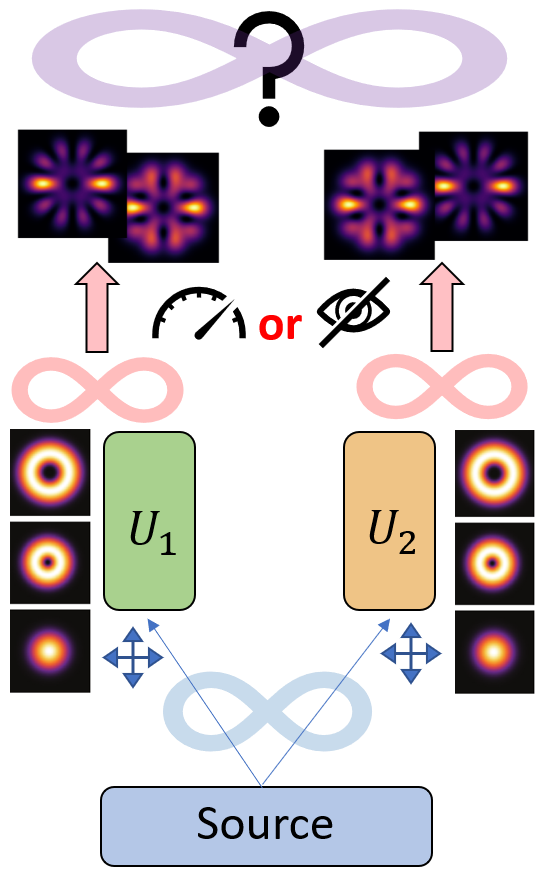
\includegraphics[scale=0.35]{concept.png}
    \caption{\textbf{Scheme of the problem.}
        The Bell state produced by a single-photon source represents the entangled input state for the two independent QWs.
        The latter evolution enlarge the space of each subsystem, creating correlation between the polarization and OAM.
        We ask for the amount of entanglement in the walkers space after \textit{i)} tracing the polarization or \textit{ii)} projecting the coins. \highlight{(not referenced (but also probably the whole figure will be changed so ok))}
    }
    \label{fig:conceptual_scheme}
\end{figure}

\section{Entanglement transfer via local projections}

\subsection{Entanglement transfer via projective measurements}

\parTitle{Problem statement}
We can formally state our problem as the following:
\begin{quote}
% \begingroup\addtolength\leftmargini{-5pt}\begin{quote}
    \textit{Given a two-photon state $\ket\Psi\in\calH$, can we find $\ket{\gamma}\in\calH^{(1)}_{\calC}$ and $\ket\delta\in\calH^{(2)}_{\calC}$ such that the entanglement in $\ket\Psi$ is optimally transferred to the projected state
    $\braket*{\gamma,\delta}{\Psi}\in\calH^{(1)}_{\calW}\otimes\calH^{(2)}_{\calW}$?}
\end{quote}%\endgroup
% In other words, we investigate whether it is possible to optimally transfer entanglement between two degrees of freedom by means of projective measurements.
A schematic description of the scenario is given in~\cref{fig:entanglement_transfer_scheme}.
It is worth stressing that, for arbitrary choices of $\ket\Psi$, such entanglement transfer is clearly impossible --- for example if $\ket\Psi$ is separable with respect to $\calH_1$ and $\calH_2$. It is therefore pivotal to figure out the conditions making such protocol viable.

\begin{figure}
    \centering
    \begin{minipage}[c]{\linewidth}
        \centering
        \begin{quantikz}
            \lstick[wires=4]{$\ket{\Psi_{\on{in}}}$}\qw &\qw & \gate[wires=2]{U_{12}}\slice{$\ket{\Psi_f}$} &\qw \\
            \qw & \gate[wires=2]{U_{23}} & & \qw\rstick{$\!\!\ket{\gamma}$}\\
            \qw & & \gate[wires=2]{U_{34}} & \qw\rstick{$\!\!\ket{\gamma}$}\\
            \qw & \qw & \qw & \qw
        \end{quantikz}
    \end{minipage}
    \caption{Entanglement transfer scheme. \highlight{(add decent description)}}
    \label{fig:entanglement_transfer_scheme}
\end{figure}

\parTitle{We are actually dealing with two problems at once}
The task at hand can be broken down into two distinct entanglement transfer problems: restricting to \emph{local} projections on both sides, the transferability of entanglement between $\calH^{(1)}_{\calC}$ and $\calH^{(1)}_{\calW}$ is independent from that between $\calH^{(2)}_{\calC}$ and $\calH^{(2)}_{\calW}$.
Most of our discussion will thus focus, without loss of generality, on the transferability on a single side.

\parTitle{Conditions for entanglement transfer}
Consider a state $\ket\Psi\in\calH$.
% , and focus on the state of the first photon: $\calH^{(1)}$.
As we only allow local operations, we have to deal with the reduced state $\rho\equiv\Tr_2\ketbra\Psi$. Projecting onto a polarization state $\ket\gamma$ then gives $\rho_{\calW}\equiv \mel\gamma\rho\gamma\in\calH^{(1)}_{\calW}$.
We want the projection $\ket\gamma$ to be such that, \textit{in the full state}, the degree of entanglement is not degraded.
For this to be the case, it is necessary and sufficient that $\rho_{\calW}$ is \textit{diagonal in the same eigenbasis of $\rho$}, and has the same eigenvalues.
More precisely, each eigenspace of $\rho$ must be invariant under the projection.
This ensures that the projection does not reveal any information about the correlations with $\calH^{(2)}$, which would damage the entanglement.
\highlight{(proper proof. Also mention that bad entanglement can be improved via local projection?)}
More explicitly, this ensures that the state
\begin{equation}
	\ket\Psi= \sum_k \sqrt{p_k} \ket{u_k}\ket{v_k}
\end{equation}
becomes
\begin{equation}
	\braket{\gamma}{\Psi} =
	\sqrt{p_{\on{proj}}}\sum_k \sqrt{p_k} \ket*{\tilde u_k}\ket{v_k}
\end{equation}
where $\ket*{\tilde u_k}\equiv \braket{\gamma}{u_k}/\sqrt{p_{\on{proj}}}$ are the post-projected states, and
$p_{\on{proj}}\equiv |\braket{\gamma}{u_k}|^2$ the projection probability.
It is worth stressing that, \emph{a priori}, the projection probabilities $|\braket{\gamma}{u_k}|^2$ depend on $k$, but we need them to be the same for optimal entanglement transfer.

\parTitle{Entanglement distillation via local projection}
The constraint on the projection probabilities can be lifted when the projection allowed in the second party is taken into consideration.
This is because any form of ``imperfect entanglement'' can be improved by means of local projections in some cases.

\parTitle{Relations with entanglement swapping}
This problem can be understood as a more restrictive version of entanglement swapping~\cite{zukowski1993eventreadydetectors}.
Entanglement swapping deals with a four-partite system $\calH_{ABCD}$, with entanglement in $\calH_{AB}$ and $\calH_{CD}$, and we wish to obtain entanglement in $\calH_{AD}$ by performing projective measurements on $\calH_{BC}$.
This is analogous to our problem, except that we only allow \emph{local} operations on $B$ and $C$. Notably, the typical solution used in the context of entanglement swapping, projecting $BC$ on a Bell state, is not available in our setting: we only allow for projections of the form $P_B\otimes P_C$.

\subsection{\texorpdfstring{$2\to N$}{2->N} entanglement transfer}

\parTitle{Problem setting}
While solving the problem in full generality is challenging, in the case of two-dimensional $\calH^{(i)}_{\calC}$ an explicit solution can be derived.
% We consider here the special case of $B,C$ being two-dimensional degrees of freedom.
Write the eigendecomposition of the reduced state $\rho\in\calH_{\calW}\otimes\calH_{\calC}$ as
\begin{equation}
	\rho= p_1 \ketbra{u} + p_2 \ketbra{v}, \,\,p_1+p_2=1.
\end{equation}
For a projection $\ket\gamma$ to preserve the invariants of $\rho$ it needs to satisfy
$\mel{u}{\PP_\gamma}{v}=0$, which is equivalent to
\begin{equation}
	\mel{\gamma}{\tr_{\calW}(\ketbra{u}{v})}{\gamma} = 0.
\end{equation}
Defining $M\equiv \tr_{\calW}(\ketbra{u}{v})$, we notice that $\tr M=0$.
Assuming $M$ is diagonalisable and $M\ket{\lambda_s}=\pm\lambda\ket{\lambda_s}$, we define
\begin{equation}
    \ket\gamma\equiv N\left(
        \ket{\lambda_+} +
        e^{i\arg\braket*{\lambda_-}{\lambda_+}} \ket{\lambda_-}
    \right),
    \label{eq:definition_projgamma_2dcase}
\end{equation}
where $N$ is a normalisation constant. Note that in general $\braket*{\lambda_+}{\lambda_-}\neq0$, as $M$ needs not be normal.
A sufficient condition for $M$ to be diagonalisable is that $\det M\neq0$, which implies that
$\{\braket*{H}{u^H},\braket*{V}{u^H}\}$ and
$\{\braket*{H}{u^V},\braket*{V}{u^V}\}$
are both linearly independent and nonzero.
\highlight{(possibly remove this paragraph, proof with SVD is better)}

\parTitle{Proof with SVD}
If $M$ is normal, then
\begin{equation}
	M = \lambda( \ketbra{v_1} - \ketbra{v_2}),
\end{equation}
for some $\lambda\in\CC$ and $\braket{v_i}{v_j}=\delta_{ij}$.
Then,
\begin{equation}
	\sqrt2\ket{\gamma_\phi} = \ket{v_1} + e^{i\phi}\ket{v_2}, \quad \phi\in\RR
\end{equation}
are suitable projections such that $\mel{\gamma_\phi}{M}{\gamma_\phi}=0$.
% The singular value decomposition of $M$ reads
% \begin{equation}
% 	M = s_1 \ketbra{v_1}{w_1} + s_2 \ketbra{v_2}{w_2},
% \end{equation}
% where $\braket{v_1}{v_2}=\braket{w_1}{w_2}=0$, $s_i\ge0$, and $\tr M=0$ translates into
% % \begin{equation}
% 	$s_1\braket{w_1}{v_1} + s_2 \braket{w_2}{v_2}=0$.
% % \end{equation}
% Consider the projections
% \begin{equation}
% \begin{aligned}
% 	\sqrt2\ket*{\gamma_\pm} &= \ket{w_1} \pm \ket{w_2}, \\
% 	\sqrt2\ket*{\gamma_\pm'} &= \ket{v_1} \pm \ket{v_2}.
% \end{aligned}
% \end{equation}
% Then clearly $\braket{\gamma_+}{\gamma_-}=\braket{\gamma_+'}{\gamma_-'}=0$, and at the same time
% \begin{equation}
% 	\mel*{\gamma_\pm}{M}{\gamma_\pm} = \mel*{\gamma_\pm'}{M}{\gamma_\pm'}.
% \end{equation}
For $M$ not normal, its SVD has the form
\begin{equation}
	M = s_1 \ketbra{u_1}{u_2} + s_2 \ketbra{u_2}{u_1}
\end{equation}
\highlight{(why??)}
with $\braket{u_1}{u_2}=0$ and $s_i>0$. Suitable projections are in this case
$\ket{\gamma_i}=\ket{u_i}$.

\section{Entanglement transfer in QWs}

\parTitle{Single step}
A single step of QW with coin $C\equiv (c_{ij})_{ij}$ amounts to the evolution
\begin{equation}
\begin{aligned}
	\ket\uparrow&\rightarrow \ket*{\Psi_\uparrow} \equiv c_{11}\ket{\uparrow,1} + c_{21}\ket{\downarrow,2}, \\
	\ket\downarrow&\rightarrow \ket*{\Psi_\downarrow} \equiv c_{12}\ket{\uparrow,1} + c_{22}\ket{\downarrow,2}.
\end{aligned}
\end{equation}
Projecting on the coin state $\ket\gamma$ we get
\begin{equation}
\begin{aligned}
	\ket*{\psi_\uparrow} \simeq \braket*{\gamma}{\Psi_\uparrow} &= \gamma_\uparrow^*c_{11}\ket1 + \gamma_\downarrow^* c_{21}\ket2, \\
	\ket*{\psi_\downarrow} \simeq \braket*{\gamma}{\Psi_\downarrow} &= \gamma_\uparrow^* c_{12} \ket1 + \gamma_\downarrow^* c_{22} \ket2.
\end{aligned}
\end{equation}
The orthogonality of these states reads
\begin{equation}
\begin{gathered}
	\braket*{\psi_\uparrow}{\psi_\downarrow}
	% \mel{\gamma}{\tr_{\calW}(\ketbra*{\Psi_\uparrow}{\Psi_\downarrow})}{\gamma}
	= |\gamma_\uparrow|^2 c_{11}^* c_{12} + |\gamma_\downarrow|^2 c_{21}^* c_{22} = 0,
\end{gathered}
\end{equation}
which is satisfied by $\sqrt2\ket\gamma = \ket\uparrow + e^{i\phi}\ket\downarrow$ for any $\phi\in\RR$.
The corresponding projection probabilities are both equal to $1/2$, as follows from
\begin{equation}
\begin{aligned}
	2\abs{\braket{\gamma}{\Psi_\uparrow}}^2 &= |c_{11}|^2 + |c_{21}|^2 = 1, \\
	2\abs{\braket{\gamma}{\Psi_\downarrow}}^2 &= |c_{12}|^2 + |c_{22}|^2 = 1.
\end{aligned}
\end{equation}
We conclude that entanglement transfer is always possible with probability $1/2$.
More precisely, if the initial state of the QW $\ket*{\Psi_{\on{in}}}$ is entangled via its coin with an external degree of freedom, as in
\begin{equation}
	\sqrt2\ket*{\Psi_{\on{in}}} = \ket{1,\uparrow} \otimes \ket{u_1} + \ket{1,\downarrow}\otimes \ket{u_2},
\end{equation}
with $\ket{u_i}$ arbitrary orthogonal states of the additional degree of freedom,
then the entanglement can always be transferred from $\calH_{\calC}$ to $\calH_{\calW}$ with probability $1/2$.
Remarkably, the freedom in the choice of the phase $\phi$ means that both $\sqrt2\ket\pm\equiv \ket\uparrow+\ket\downarrow$ are \emph{both} suitable projections achieving entanglement transfer.
This result in an overall transfer success probability of $1$: both outcomes of measuring in the $\ket\pm$ basis achieve entanglement transfer, albeit with different post-measurement states.

\parTitle{Multiple steps}
After multiple QW steps, the output state has the form
\begin{equation}
\begin{aligned}
	\ket{\Psi_s} =
	\cos(\theta_s) \ket{\uparrow,\Psi_{s,\uparrow}} +
	\sin(\theta_s) \ket{\downarrow,\Psi_{s,\downarrow}},
	% s\in\{\uparrow,\downarrow\}.
\end{aligned}
\end{equation}
where $\theta_s$ and $\ket{\Psi_{s,p}}$ depend on the number of steps and choice of coin operators.
To achieve entanglement transfer, we consider the matrix
$M\equiv \tr_{\calW}(\ketbra{\Psi_\uparrow}{\Psi_\downarrow})$,
which equals
\begin{equation}\scalebox{0.97}{$\displaystyle
	M = \begin{pmatrix}
		\cos(\theta_\uparrow)\cos(\theta_\downarrow) \calO_{\uparrow\uparrow} &
		\cos(\theta_\uparrow)\sin(\theta_{\downarrow}) \calO_{\downarrow\uparrow} \\
		\cos(\theta_\downarrow)\sin(\theta_{\uparrow}) \calO_{\uparrow\downarrow} &
		\sin(\theta_\uparrow)\sin(\theta_\downarrow) \calO_{\downarrow\downarrow}
	\end{pmatrix}.
$}\end{equation}
where
$\calO_{sp}\equiv\braket{\Psi_{\downarrow s}}{\Psi_{\uparrow p}}$.
This $M$ is not in general Hermitian, nor normal. Consequently, while it is possible to find a projection $\ket\gamma$ via~\cref{eq:definition_projgamma_2dcase}, the projection probabilities are not in general equal.
This can be fixed by either choosing coin operations which make these probabilities equal \highlight{(probably not possible)}, or by compensating the unequal projection probabilities with similar projection probabilities on the other party.


\parTitle{Pair of QWs}
Up to now we focused on the transferability between coin and walker degrees of freedom of a single QW.
However, the same reasoning apply symmetrically if the additional party the first QW is entangled to is another QW.
In particular, we can consider a scheme in which the initial state is a pair of entangled coins (\emph{e.g.} the polarisations of a pair of photons) in a single state
\begin{equation}
	\sqrt2\ket{\Psi_{\calC}}\equiv \ket{\uparrow,\downarrow} + \ket{\downarrow,\uparrow}.
\end{equation}
Then, applying the same QW evolution on both sides, we have a state of the form
\begin{equation}
	\sqrt2(\calU_{\on{QW}}\otimes \calU_{\on{QW}}) \ket{\Psi_{\calC}} =
	\ket{\Psi_\uparrow,\Psi_\downarrow} +
	\ket{\Psi_\downarrow,\Psi_\uparrow}.
\end{equation}
The reduced states on $\calH^{(1)}$ and $\calH^{(2)}$ are thus both equal to
% \begin{equation}
	$2\rho = \PP_{\Psi_\uparrow} + \PP_{\Psi_\downarrow}$,
% \end{equation}
and the transferability conditions become
\begin{equation}
	\mel{\gamma}{\tr_{\calW}(\ketbra{\Psi_\uparrow}{\Psi_\downarrow})}{\gamma} = 0.
\end{equation}
We can always find two orthogonal projections $\ket{\gamma_i}$, $i=1,2$ that satisfy this condition, as shown previously.
The post-selected state is therefore
\begin{equation}
	\braket*{\gamma^{(1)}}{\Psi_\uparrow}\otimes \braket*{\gamma^{(2)}}{\Psi_\downarrow}
	+
	\braket*{\gamma^{(1)}}{\Psi_\downarrow}\otimes \braket*{\gamma^{(2)}}{\Psi_\uparrow}
\end{equation}
with $\ket*{\gamma^{(i)}}$ the projection used on the $i$-th QW.


\subsection{Remove?}
Consider the following scenario: two polarisation-entangled photons evolve independently with the same unitary $\mathcal U$, which entangles their polarisation and OAM degrees of freedom. After the evolution, the polarisations are projected. Is it possible with such a scheme to transfer the polarisation entanglement into the OAMs?

Suppose the two photons are initially the state
\begin{equation}
    \ket{\on{initial}}\equiv
    (a_{p_0,\ell_0,H}^\dagger
    a_{p_1,\ell_0,V}^\dagger +
    a_{p_0,\ell_0,V}^\dagger
    a_{p_1,\ell_0,H}^\dagger) \ket{\mathrm{vac}},
    \label{eq:proj_initial_state}
\end{equation}
for some initial OAM $\ell_0$, and with $p_i, i=0,1$ the $i$-th position.
Note that~\cref{eq:proj_initial_state} is nothing but a state of the form $\ket{HV}+\ket{VH}$ in second quantisation notation.
As long as no operation interfering the two photons is used, we can safely operate in this bra-ket notation.
Evolving the photons locally with the same unitary $\calU$ gives
$(\calU\otimes\calU)(\ket{HV}+\ket{VH})$.
Let us then define
$\ket{\Psi^s}\equiv\calU\ket s$, with $s\in\{H,V\}$.
The states $\ket{\Psi^s}$ are one-photon states which in general display entanglement between their polarisation and OAM degrees of freedom:
\begin{equation}
    \ket{\Psi^s}=
    \cos\theta_s \ket H\otimes\ket{\Psi^s_{H}} +
    \sin\theta_s \ket V\otimes\ket{\Psi^s_{V}},
\end{equation}
for some angle $\theta_s$ and states $\ket{\Psi^s_p}$.

\section{Purity of reduced states}
\label{sec:purity_reduced_states}

\begin{figure*}[t]
    \centering
    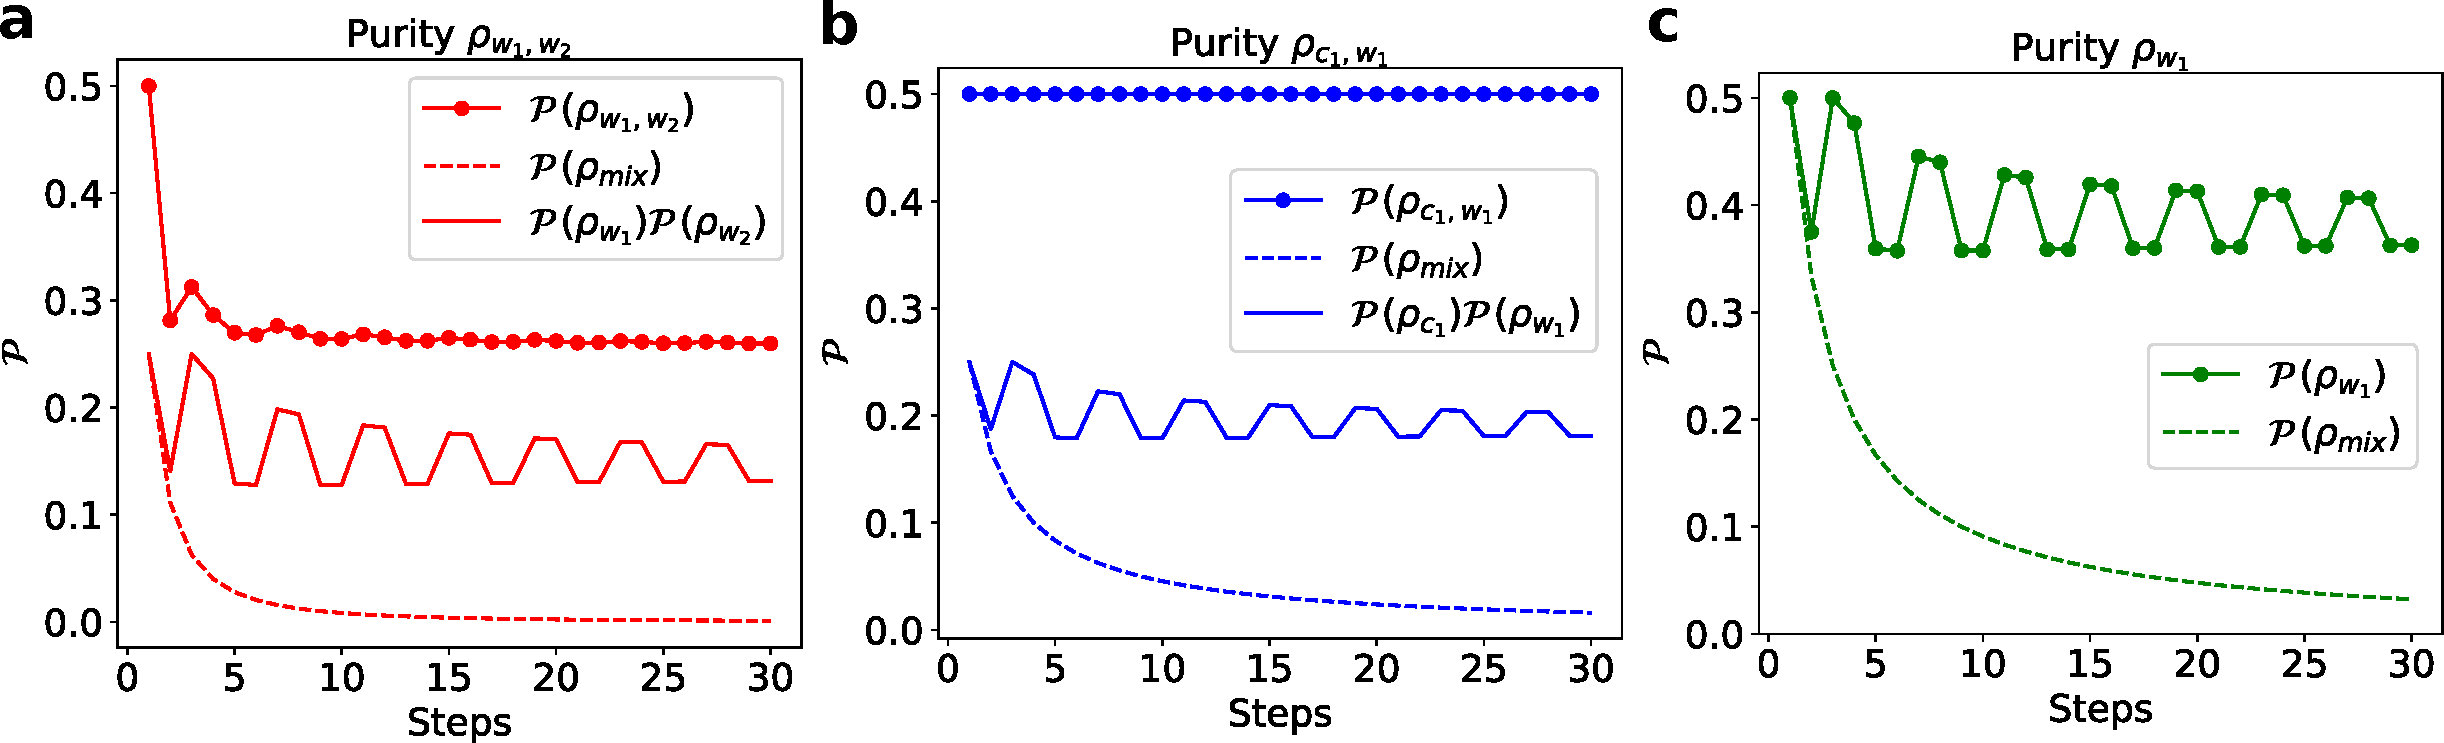
\includegraphics[width=\textwidth]{purity_of_reduced_states.pdf}
    \caption{\textbf{Purity of traced subsystems}.
    In each panel we report the purity of the state for different number of steps, of two identical Hadamard quantum walks. The dashed line correspond to the purities of the classical statistical mixture associated to the subspace after investigation.
    \highlight{(I don't understand what $\rho_{\on{mix}}$ represents. It should also probably be mentioned in the text.)}\\
    \highlight{(Mention why we include the product of purities as well.)}\\
    \highlight{(why do only the upper lines use dots? I would add dots (or other marker) on all lines (or none))}\\
    \highlight{(comment on the peculiar zigzagging behaviours)}
    }
    \label{fig:purity_traced_subsystems}
\end{figure*}

\parTitle{Why do we do this?}
The state purity of the traced subsystem could provide a first insight on the entanglement structure of the state. \highlight{(we should probably justify this a bit more)}

\parTitle{What exactly are we computing}
We study here the purity of reduced states at different stages of a Hadamard QW evolution \highlight{(define what this is (if not done before), and comment why we use \textit{Hadamard} QW)}.
More specifically, we consider the purities of
\begin{enumerate}
    \item the walkers' states $\rho_{w_1,w_2}=\tr_{c_1,c_2}(\rho)$,
    \item a single particle's state: $\rho_{w_1,c_1}\equiv\tr_{c_2,w_2}(\rho)$,
    \item a single walker's state $\rho_{w_1}\equiv\tr_{c_1,w_2,c_2}(\rho)$.
\end{enumerate}
Each quantity is computed on the outputs of the Hadamard QW after different numbers of steps, as reported in~\cref{fig:purity_traced_subsystems}
\highlight{(justify why these particular choices (e.g. why not also $\rho_{c_1}$?)}
% In~\cref{fig:purity_traced_subsystems} we report the purities $\calP\equiv \tr(\rho^2)$) for increasing steps of an Hadamard QW for the following states. Given $\rho^f = \ket{\Psi^f}\bra{\Psi^f}$, we consider the joint walkers state, tracing the polarization $\rho_{w_1,w_2}= \tr( \rho^f)_{c_1,c_2}$, the state of a single quantum walk tracing the other one $\rho_{c_1,w_1}= \tr( \rho^f)_{c_2,w_2}$ and the state of a single walker tracing the remaining subsystems $\rho_{w_1}= \tr( \rho^f)_{c_1,c_2,w_2}$.
If $\rho_{w_1,w_2}=\rho_{w_1}\otimes\rho_{w_2}$, then $\mathcal{P}(\rho_{w_1,w_2}) = \mathcal{P}(\rho_{w_1}) \mathcal{P}(\rho_{w_2})$, where $\calP(\rho)\equiv\tr(\rho^2)$ denotes the purity of the state.
In~\cref{fig:purity_traced_subsystems}a we show that $\calP(\rho_{w_1,w_2})>\calP(\rho_{w_1})\calP(\rho_{w_2})$, and similarly for $\rho_{c_1,w_1}$,
revealing the presence of residual correlations between walkers, and between the internal degrees of freedom of the individual particles \highlight{(these can be purely classical correlations though. The purity not being factorisable only rules out product states, not separable ones. Consider \textit{e.g.} $(\ketbra{00}+\ketbra{11})/2$)}.
This is further confirmed by the negativities reported in~\cref{fig:neg_trace}a.


\parTitle{Results for general case}
We then consider the most general cases, namely two different unitaries transformation made by random step-dependent coin operators. In~\cref{fig:neg_trace}b and c we report the histograms for the negativities of $\rho_{w_1,w_2}$ and $\rho_{c_1, w_1}$, computed on samples of $1000$ pairs of random unitaries $(U_1,U_2)$ \highlight{(how were these sampled? uniformly random or something else?)}, for different step numbers. The histograms seem to become more peaked around higher values of negativities with increasing numbers of steps \highlight{(meaning...?)}.

\parTitle{What did we conclude from this?}

\begin{figure*}[hbt]
    \centering
    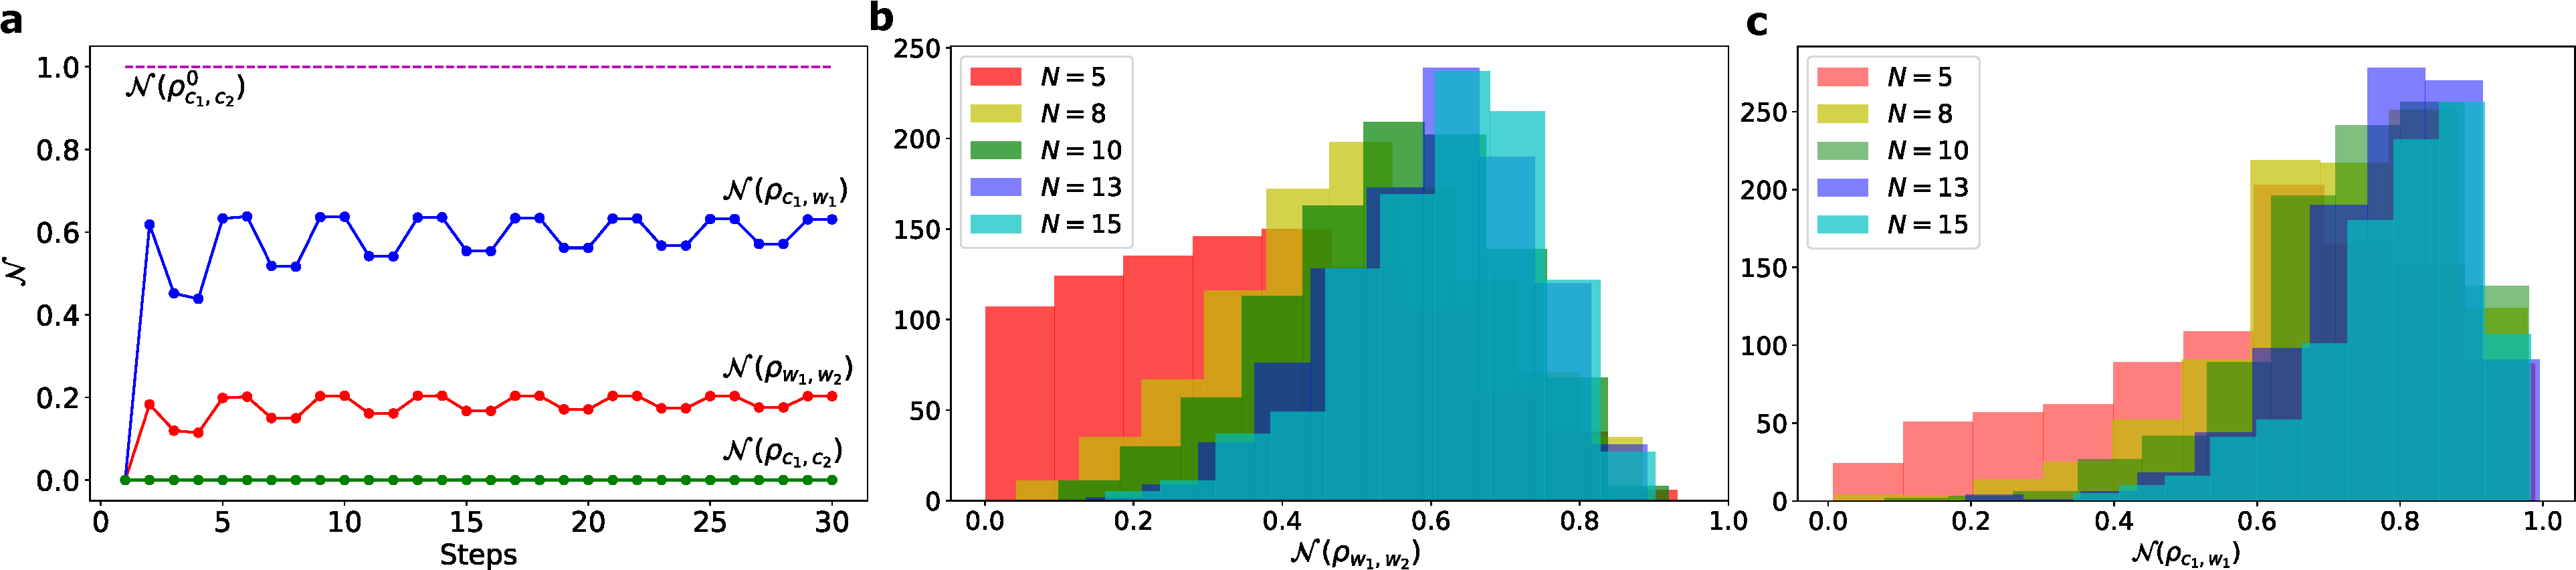
\includegraphics[width=\textwidth]{negs+rand.pdf}
    \caption{\textbf{Negativity criterion}.
    (a) Negativity, at each step of the Hadamard QWs, of different reduced states.
    % We consider in red the subsystems associated to the two walkers positions $(w_1,w_2) $ tracing the two coin, in green the system of the two coin tracing the positions $(c_1, c_2)$ and in blue the system of a single quantum walker tracing the other one, namely $(c_1, w_1)$ in the plot.
    In magenta (dashed line) we report for reference the negativity of the initial Bell state in the coin degree of freedom.
    We observe a non-zero negativity between the two walkers. (b-c) Negativities of $\rho_{w_1, w_2}$ and $\rho_{c_1, w_1}$ computed for $1000$ random unitaries. Relaxing the condition of identical QWs and allowing the coin to change at each step, higher values of negativities can be obtained. Furthermore the average increases with the number of step.}
    \label{fig:neg_trace}
\end{figure*}



\section{Projected states, numerical results}
\label{sec:projected_states}

\parTitle{What do we do here and why}
In~\cref{sec:projected_states} we showed that reduced states are entangled.
We here investigate the entanglement properties when \textit{projecting} the coins. While making the scheme probabilistic, this will allow for far improved entanglement transfer results \highlight{(I think?)}.
% Now we look for saturating the bound, projecting the coin on suitable directions.

Fix a basis $\ket{\gamma_1},\ket{\gamma_2}$ for the polarization and consider the associated projectors
$\PP_{ij}\equiv \ketbra{\gamma_i}\otimes\ketbra{\gamma_j}$.
Applying these to an initial state of the form
$\alpha\ket{\Psi_\uparrow\Psi_\downarrow}+\beta\ket{\Psi_\downarrow\Psi_\uparrow}$
gives
\begin{equation}
    \alpha\ket*{\Psi_\uparrow^i\Psi_\downarrow^j} +
    \beta\ket*{\Psi_\downarrow^i\Psi_\uparrow^j}.
\end{equation}


% \parTitle{Notation?}
% First, let us define a generic coin projectors, starting from the orthonormal basis
% \begin{equation}\begin{aligned}
%     \ket{0} &= \cos{\frac{\theta}{2}} \ket{\uparrow}+ 
%     e^{i\phi}\sin{\frac{\theta}{2}}\ket{\downarrow} \\
%     \ket{1} &= \sin{\frac{\theta}{2}} \ket{\uparrow}-
%     e^{i\phi}\cos{\frac{\theta}{2}}\ket{\downarrow}
% \end{aligned}\end{equation}
% \highlight{(are we using this definition somewhere? Also if we need to defined these, I'd use a different notation highlighting the $\theta,\phi$ dependence)}

% where $\theta \in [0, \pi ]$ and $\phi \in [0, 2\pi]$. We then define the four projectors for two separable measurements on the two coin subspace as
% \begin{equation}
%     \hat{P}_{lm}(\theta, \phi) =
%     \hat{P}_{l}(\theta, \phi) \otimes \hat{P}_{m}(\theta, \phi) =
%     \ketbra{lm},
% \end{equation}
% with $l,m \in\{0,1\}$ the two possible coin states \highlight{(explicit phase dependence in $\ell,m$)}.
% Applying these operators on the state in~ \cref{eq:final_state} we obtain in the $(w_1, w_2)$ subspace the states
% \begin{subequations}
% \label{eq:prj_state}
% \begin{align}
%     \hat{P}_{00} &\rightarrow \alpha_{00}\ket{\psi^{0 \uparrow}_1 \psi^{0 \downarrow}_2} + \beta_{00}\ket{\psi^{0 \downarrow}_1 \psi^{0 \uparrow}_2} \label{eq:prj_state_a}\\
%     \hat{P}_{01} &\rightarrow \alpha_{01}\ket{\psi^{0 \uparrow}_1 \psi^{1 \downarrow}_2} + \beta_{01}\ket{\psi^{0 \downarrow}_1 \psi^{1 \uparrow}_2}\label{eq:prj_state_b}\\
%     \hat{P}_{10} &\rightarrow \alpha_{10}\ket{\psi^{1 \uparrow}_1 \psi^{0 \downarrow}_2} + \beta_{10}\ket{\psi^{1 \downarrow}_1 \psi^{0 \uparrow}_2}\label{eq:prj_state_c}\\
%      \hat{P}_{11} &\rightarrow \alpha_{11}\ket{\psi^{1 \uparrow}_1 \psi^{1 \downarrow}_2} + \beta_{11}\ket{\psi^{1 \downarrow}_1 \psi^{1 \uparrow}_2}\label{eq:prj_state_d}.
% \end{align}
% \end{subequations}

% In the above expression the wavefuctions $\psi^{lk}_i$ are the result of the projection along $l$ of the output state $\ket{\Psi^{k}_i}$, namely the state after the single particle quantum walk $U_i$, with $k$ as initial coin.

\begin{figure*}[t]
    \centering
    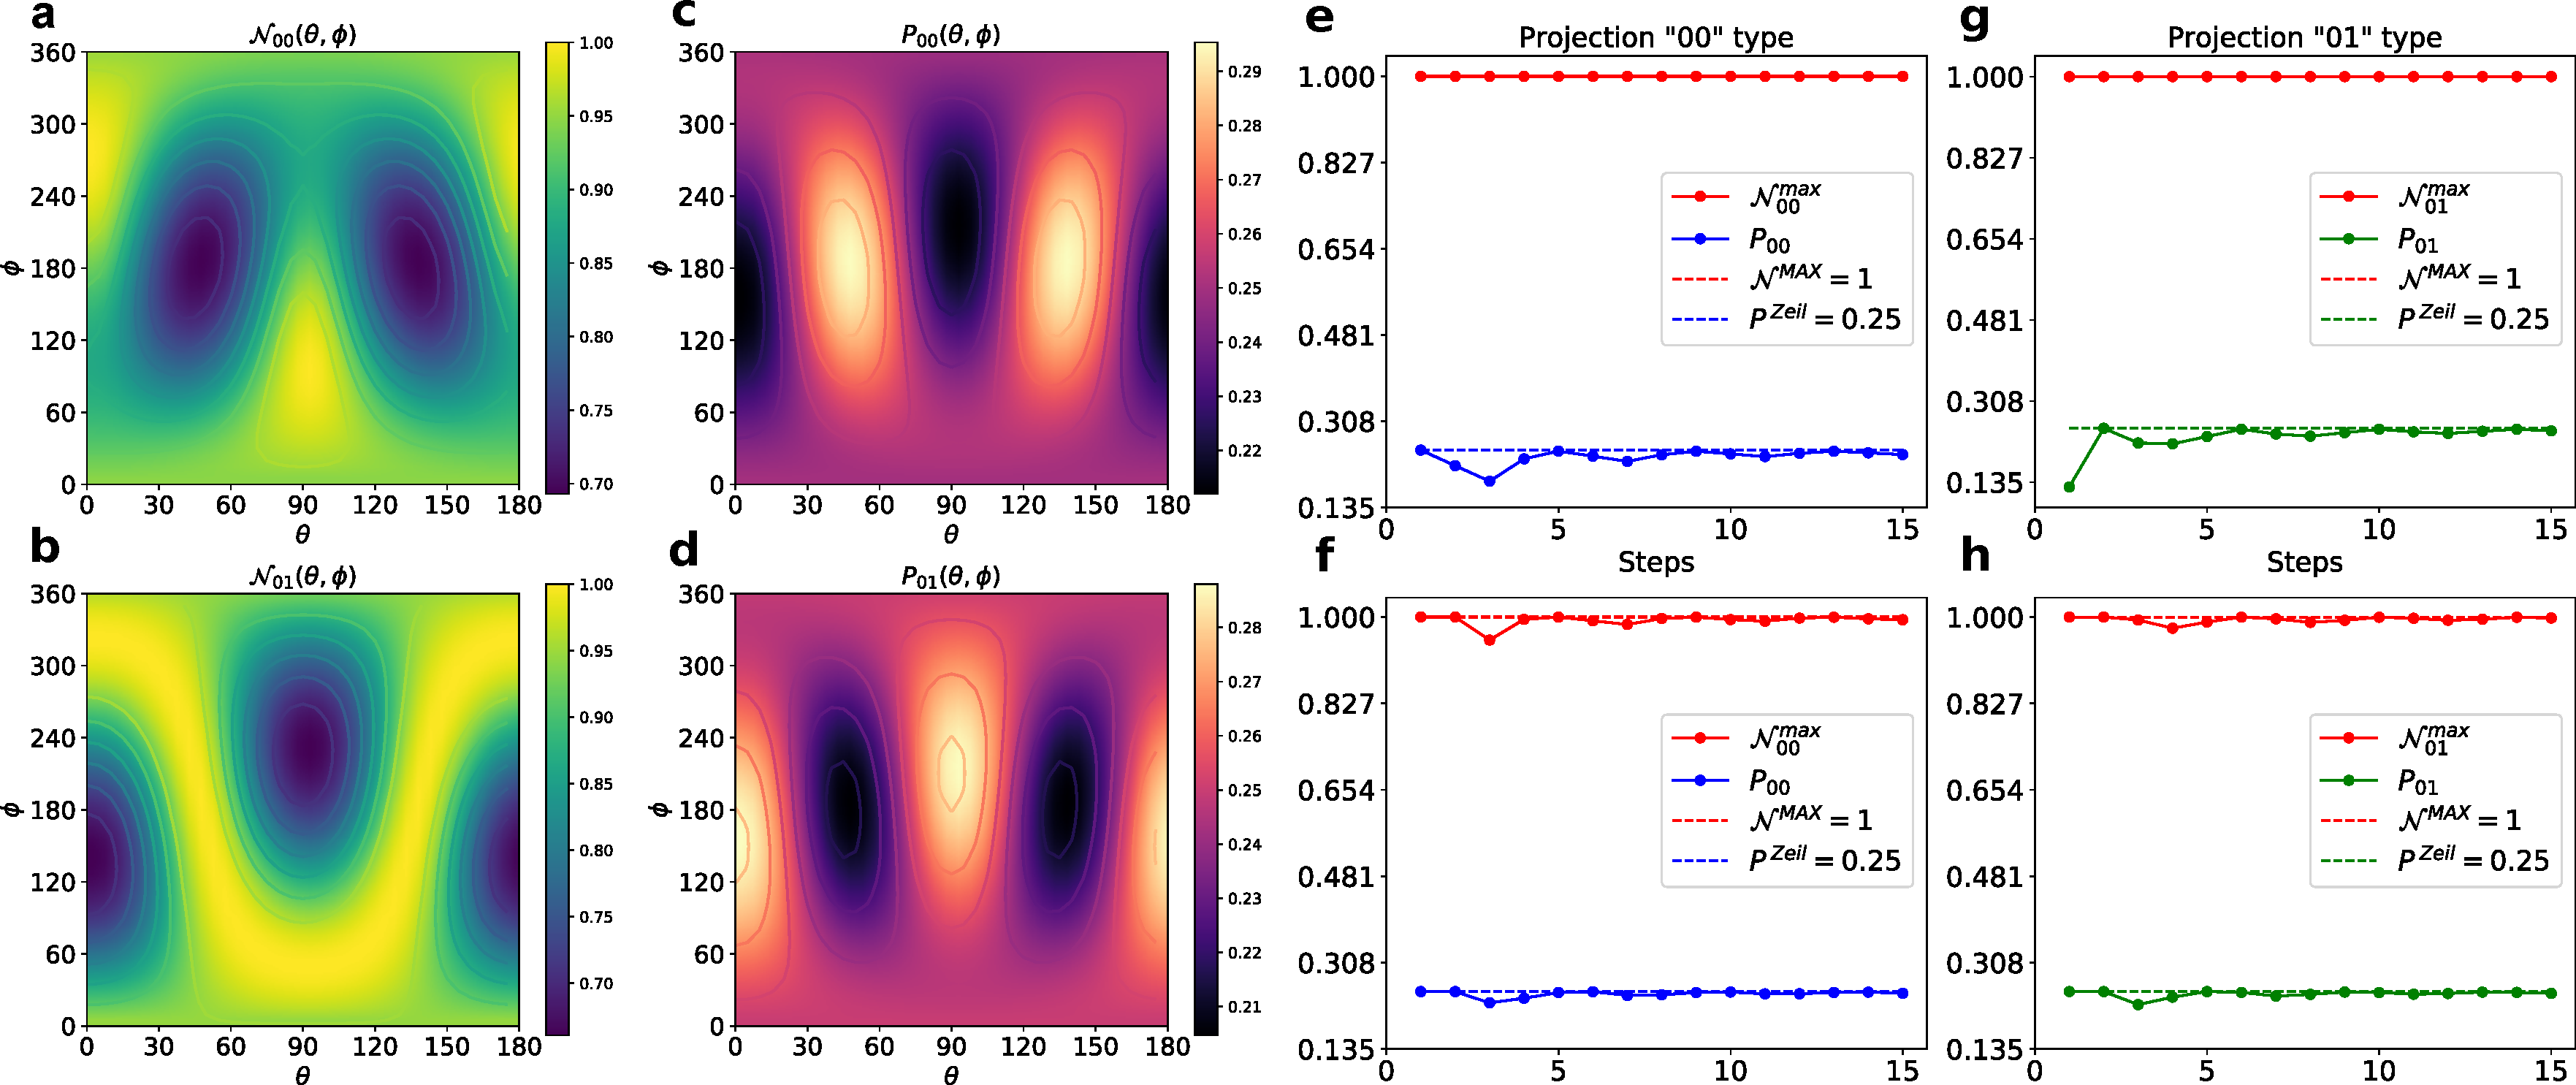
\includegraphics[width=\textwidth]{proj.pdf}
    \caption{\textbf{Projection optimization for Hadamard quantum walks.} a-b) State negativities for different type of projection $00$ and $01$ (the other two cases display the same behaviour)in terms of $(\theta, \phi)$. It is worth to note that $\mathcal{N}_{lm}>0.6$ in both cases. c-d) Corresponding surface for the projection probabilities. It is possible to obtain $P_{lm}> 0.25$ (generation probability of Ref \cite{fickler2012quantum}) but with non-optimal negativity. e-f) $\mathcal{N}_{00}$ and $P_{00}$ respect with different number of steps in the case e) of $\mathcal{N}_{00}$ optimization and f) for the maximization of both $\mathcal{N}_{00}$ and $P_{00}$. We note that both bound ($1, 0.25$) can be saturated by our protocol. g-h) same calculation of panels e-f) for $01$ projection.}
    \label{fig:10steps_results}
\end{figure*}

\parTitle{Case with same QW on both sides}
We firstly investigate, as in~\cref{sec:purity_reduced_states}, the case $U_1 = U_2$. The states in \cref{eq:prj_state_a} and  \cref{eq:prj_state_d} can be rewritten as $\alpha \ket{\psi_a \psi_b} + \beta \ket{\psi_b \psi_a}$, since only two type of qudits can be obtained.
In the literature such states have been demonstrated exploiting the entanglement of a Bell state in polarization qubits which is transferred to a state in the orbital angular momentum (OAM) \highlight{(reference)}.
In such apparatus, the two QWs are replaced by Sagnac interferometers with one spatial light modulator on each side displaying two holograms $\{\psi_a, \psi_b\}$~\cite{fickler2012quantum} \highlight{(might be useful to add a couple sentences on what holograms are etc)}. The resulting state is similar to~\cref{eq:final_state} but with single particle states in which polarization and OAM are separable, i.e $\ket{\Psi^{Zeil}}=A(\ket{\uparrow \psi_a}\ket{\downarrow \psi_b} +\ket{\downarrow \psi_b} \ket{\uparrow \psi_a})$ \highlight{(explain better this definition, which doesn't seem to be used again later)}.
Despite the similarities of the two techniques \highlight{(which two techniques?)} it is worth noting that this state cannot display the same properties under coin tracing\highlight{(?)}.
Indeed in the case of $\braket{\psi_a}{\psi_b}=0$, which ensure the maximum negativity when the state is projected with $\hat{P}_{00}(90\degree,0)$, does not display entanglement when the polarization is traced (the state is a statistical mixture of $\{\psi_a, \psi_b\}$).
Furthermore if we look at the states of~\cref{eq:prj_state_b} and~\cref{eq:prj_state_c}, they need in general four type of qudits to be described even with two identical unitaries. These states could be reproduced by the apparatus of Ref. \cite{fickler2012quantum} but with at least four holograms.
\highlight{(the message of this paragraph is not clear)}

\parTitle{Look for projections maximizing negativity on reduced state}
We now test the capability of our setup \highlight{(is this referring to the \textit{experimental} setup, or to the type of dynamics being considered here?)} to generate states
% in~\cref{eq:prj_state}
with maximal negativity, in the case of two identical Hadamard QWs. We look for optimal $(\theta, \phi)$ parameters maximizing both the negativity and the projection probability. We find two sets \highlight{(what kind of sets? Are these single values or range of possible values?)} that maximize these quantities for the projections types $\{00, 11\}$ and $\{01, 10\}$ respectively \highlight{(clarify what "projection type" means here)}.
In~\cref{fig:10steps_results}a,b we report the value of negativities and projection probabilities in terms of the two parameters for $N=10$ steps. It is worth noting the existence of large areas in which $\mathcal{N}_{lm}$ assumes the value 1. In the panels e-h of~\cref{fig:10steps_results} we report the values of $\mathcal{N}_{lm}$ and $\mathcal{P}_{lm}$ for any step for both set of optimal parameter, when the maximization is performed \textit{i)} on the negativity and \textit{ii)} both the negativity and projection probabilities. In particular we compare the latter with the generation probability of Ref. \cite{fickler2012quantum}.
Same results can be obtained with randomly sampled quantum walks: it is always possible to find optimal projectors to retrieve the ebit \highlight{(ref if we want to use this terminology)} of entanglement in the two walkers state.

\parTitle{Different unitaries} \highlight{We say above "\textit{We firstly investigate the case $U_1=U_2$}", but where do we investigate other cases?}

\section{Entanglement accumulation}

Here we ask if it could be possible to accumulate more than one ebit of entanglement in the walkers spaces, iterating the two parallel QWs protocol. After the first round and the optimal projection of the coin, the output is one of the states of \cref{eq:prj_state}. Since the coin and walkers position are now separable again, as in the previous input states, one can generated a new Bell state in the coin degree of freedom. Such operation can be performed with an Hadamard gate on the first qubit, followed by C-NOT operation, $U^{Bell} = U_{CNOT}*(H_1 \otimes I_2)$.

Let us consider the case in which for simplicity the first projection is 00 type and the unitaries are identical. The input state for the second iteration, after the $U^{Bell}$ on the coin
\begin{align}
     \ket{\Psi^{0 (1)}} &= \frac{1}{2}\left(\ket{\uparrow \psi_a}_1 \ket{\uparrow \psi_b}_2 +\ket{\uparrow \psi_b}_1 \ket{\uparrow \psi_a}_2 + \right. \notag\\
      &\left. + \ket{\downarrow \psi_a}_1 \ket{\downarrow \psi_b}_2 +
     \ket{\downarrow \psi_b}_1 \ket{\downarrow \psi_a}_2
     \right),
\end{align}
injected to the others QWs, will produce the state
\begin{align}
     \ket{\Psi^{f(1)}} &=
     \alpha \ket{\Psi^{\uparrow \psi_a}_1\Psi^{\uparrow \psi_b}_2} +
     \beta \ket{\Psi^{\uparrow \psi_b}_1\Psi^{\uparrow \psi_a}_2} +  \notag \\
        &+ \delta \ket{\Psi^{\downarrow \psi_a}_1\Psi^{\downarrow \psi_b}_2} 
         + \gamma \ket{\Psi^{\downarrow \psi_b}_1\Psi^{\downarrow \psi_a}_2}.
\label{eq:final_state1}                 
\end{align}

\begin{figure}[t]
\centering
    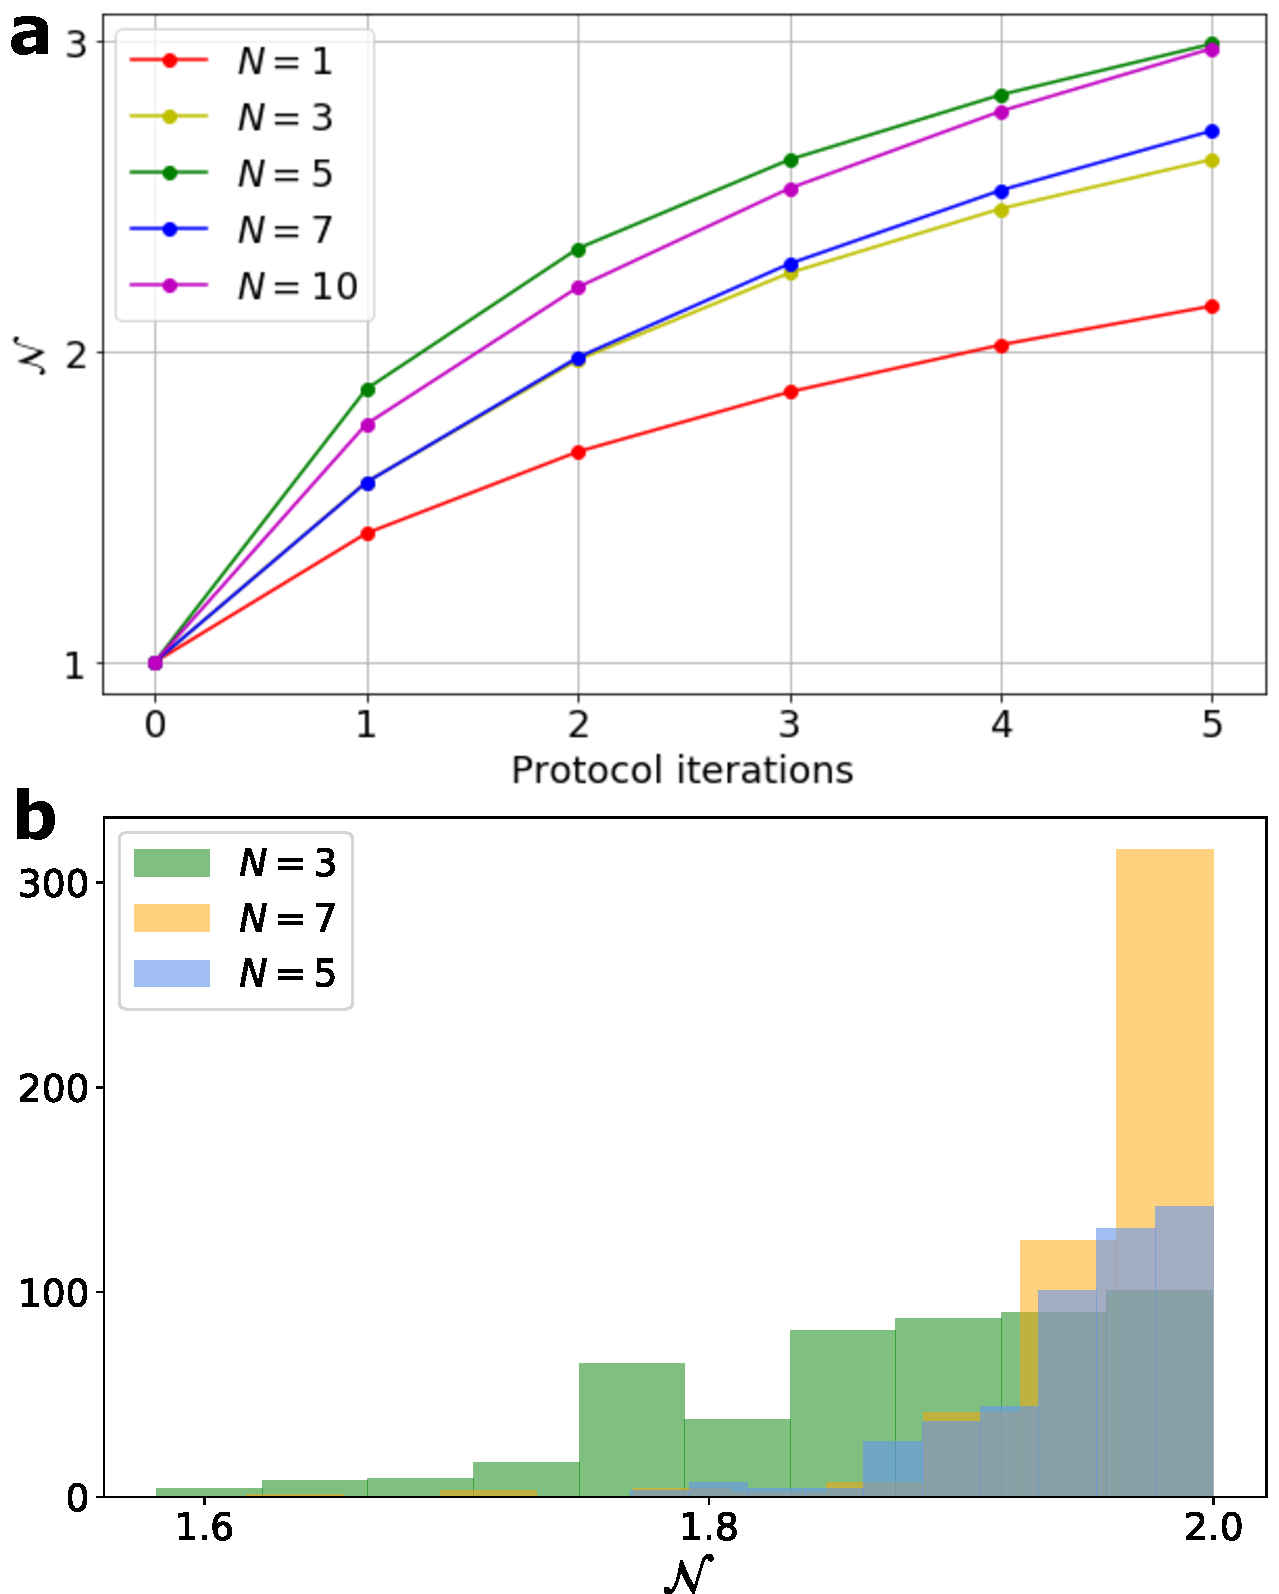
\includegraphics[width = \columnwidth]{figures/scaling.pdf}
    \caption{\textbf{Entanglement accumulation} a) Trend of the entanglement accumulation after several iterations of the protocol with identical Hadamard QW of $N=\{1,3,5,7,10\}$ steps. From such simulation seems that the optimal transfer of one ebit per iteration cannot be reached. However, relaxing the need to have same unitaries at each step, the optimal scaling can be obtained. b) Histograms for one iteration of entanglement transfer protocol (the stage zero with two identical Hadamard QWs), for three values of QW steps per iteration $N=\{3,5,7\}$. 
    Each histograms represent the distribution of $500$ random extracted coin operators for individuating the QW unitary to apply to the two walkers in the state $\ket{\Psi^{0(1)}}$. We observe that it is possible to find unitary operation for the second entanglement transfer which allows to saturate the bound of 2 ebit of entanglement. In particular histograms tend to pick towards 2 with increasing number of steps. All the calculations were performed considering coin projection of type $00$.}
    \label{fig:ent_acc}
\end{figure}
It is clear that after a further coin projection, the whole state will collapse in a superposition of four terms with at least four different qudits states involved.
Due to the high-dimension of the two walkers position, we can generate states in which the four qudits in the superposition are mutually orthogonal. To be more precise,
let us consider, as example, a state $\ket{q} = \sum_{s =1}^{n_q} \ket{ss}$, where $s$ are the walkers position. The negativity of such state scales as $\log_2(n_q + 1)$. According to such intuition we expect that the maximum negativity of the state $\ket{\Psi^{f(N_i)}}$ at the iteration $N_i$ after a proper coin projection, could be $\mathcal{N}^{Max} =\log_2( 2^{N_i}+1)$. Indeed the number of states in the superposition grows as $2^{N_i}$, as can be verified looking at \eqref{eq:final_state} and \eqref{eq:final_state1}.

In Fig. \ref{fig:ent_acc}a we report numerical simulation on the scaling of negativity according to increasing number of iteration. We consider cascaded Hadamard QWs, starting from the initial state in \eqref{eq:initial_state}, with $U^{Bell}$ coin operation in between. We focus on iteration in which the optimization on the negativity is performed on projectors of type $00$, after Qws of equal steps $N$, for different value of $N$. According to this simulation, the optimal curve $\mathcal{N}^{Max}$ is not saturated. For improving the performance of the protocol different strategies can be investigated. In 
Fig. \ref{fig:ent_acc}b we try to change the unitary after the first optimal coin projection on two Hadamard QWs. To this aim 
we have random sampled the coin operators for the next QWs evolution, considering the accumulation after one iteration of the protocol for different steps. From such simulation turns out that there is a dependence both from the choice of the unitary in the second stage and from the number of steps of each QW (see Fig. \ref{fig:ent_acc}b). The latter is not surprising since with high number of steps we cover higher dimensional Hilbert spaces and, consequently, it could be easier to produce four qudits mutually orthogonal inside the state produced by the projection of the coins in $\ket{\Psi^{f(1)}}$.








%It is clear that after a further coin projection, the whole state will collapse in a superposition of four terms with at least four different qudits states involved.
%Due to the high-dimension of the two walkers position, we can generate states in which the four qudits in the superposition are mutually orthogonal (states which display one ebit of entanglement present four qudits entangled too, see previous expression \cref{eq:prj_state}).
%Let us consider a state $\ket{q} = \sum_{s =1}^{n_q} \ket{ss}$, where $s$ are the walkers position. The negativity of such state (normalized to the ebit) scales as $n_q - 1$. According to such intuition we expect that the maximum negativity of the state $\ket{\Psi^{f(N_i)}}$ at the iteration $N_i$ after a proper coin projection, is at least $\mathcal{N}^{Max} = 2^{N_i}-1$. Indeed the number of states in the superposition grows as $2^{N_i}$, as can be verified looking at \cref{eq:final_state} and \cref{eq:final_state1}.

%In \Cref{fig:ent_acc} we report numerical simulation on the scaling of negativity according to increasing number of iteration. We consider cascaded Hadamard QWs, starting from the initial state in \cref{eq:initial_state}, with $U^{Bell}$ coin operation in between. We focus on iteration in which the optimization on the negativity is performed on projectors of type $00$ and $01$, after Qws of equal steps $N$, for different value of $N$. According to this simulation, the optimal curve $\mathcal{N}^{Max}$ is not saturated. For improving the performance of the protocol different strategies can be investigated: using different unitaries at each iteration, projecting on two different single coin measurement, i.e. optimizing on 4 parameters, or varying the number of steps at each iteration.



\subsection{A proof-of-principle experiment}
Here we propose a scheme for the realization of the entanglement accumulation protocol in a photonic platform that encodes coin and walkers position in polarization and OAM degree of freedom. This proposal provides the realization of two iterations, giving access to states with 2 ebit of entanglement. 

The scheme works as follows. It requires that at first iteration the two Qws are identical and to perform type 00 projection on the coins. In this way, the state after the projection that maximize the negativity will be $1/\sqrt{2}\ket{\uparrow \uparrow}\otimes(\ket{\psi_a\psi_b}\pm\ket{\psi_b\psi_a})$. 
It is straightforward to show that the action of a polarizing beam-splitter combined with two half waveplates can perform with probability $1/2$ the $U^{Bell}$ needed to perfom the accumulation.
Indeed, rewriting the state in terms of creation operators we have:
\begin{equation}
    \frac{1}{\sqrt{2}}\left(a^{\dagger}_{\uparrow, \psi_a,1}a^{\dagger}_{\uparrow, \psi_b,2}+a^{\dagger}_{\uparrow, \psi_b,1}a^{\dagger}_{\uparrow, \psi_a,2} \right)\ket{0} 
    \label{eq: snd_quant}
\end{equation}
The two photon are injected in the two input port of a polarizing beam-splitter, after a polarization rotation made by two half-waveplate (see \Cref{fig:exp_ent_acc}). Then creator operators in \cref{eq: snd_quant} become

\begin{equation}\begin{aligned}
    a^{\dagger}_{\uparrow, \psi_{a/b},1} & \rightarrow \cos{\theta_1}a^{\dagger}_{\uparrow, \psi_{a/b},1} + i\sin{\theta_1}a^{\dagger}_{\downarrow, \psi_{a/b},2} \\
    a^{\dagger}_{\uparrow, \psi_{a/b},2} & \rightarrow \cos{\theta_2}a^{\dagger}_{\uparrow, \psi_{a/b},2} + i\sin{\theta_2}a^{\dagger}_{\downarrow, \psi_{a/b},1}
\end{aligned}\end{equation}

\begin{figure}[t]
    \centering
    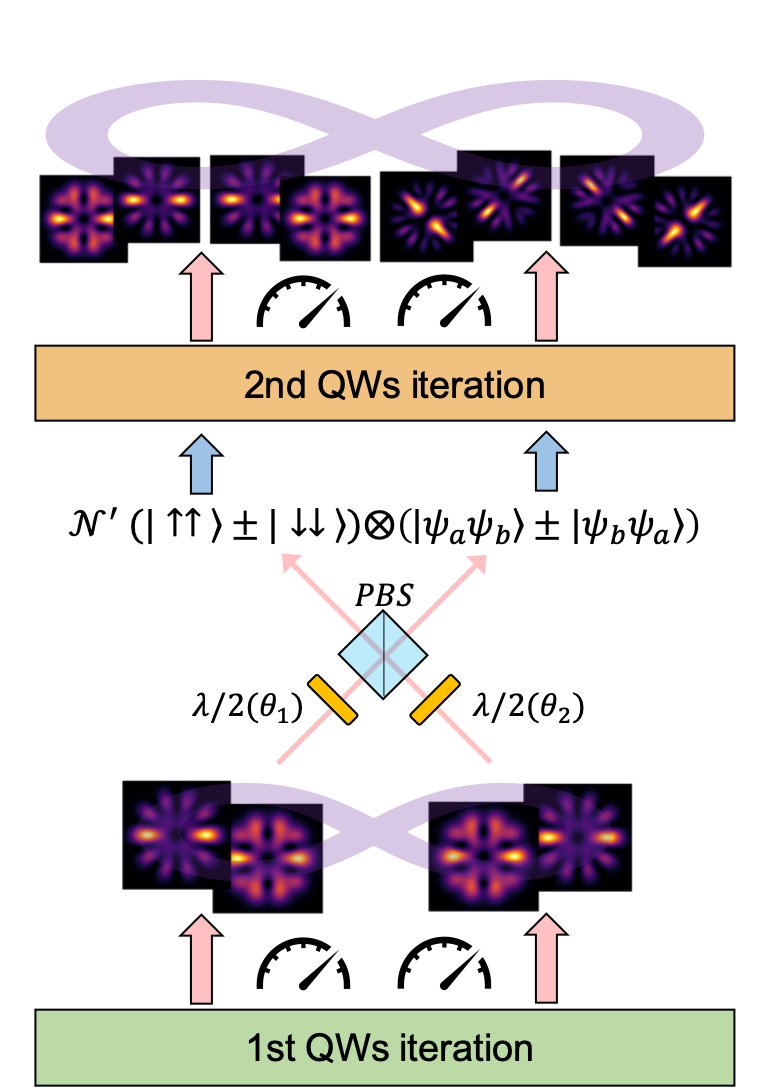
\includegraphics[scale= 0.45]{exp_ent_acc.png}
    \caption{\textbf{Experimental proposal}}
    \label{fig:exp_ent_acc}
\end{figure}


Substituting such expression in \cref{eq: snd_quant} and considering $\theta_1 = \theta_2$ we obtain 
\begin{align}
\frac{1}{2}& * \frac{\left( \ket{\uparrow \uparrow} \pm
\ket{\downarrow \downarrow}\right) }{\sqrt{2}}\otimes \frac{\left( \ket{\psi_a \psi_b} \mp
\ket{\psi_b \psi_a}\right) }{\sqrt{2}} +\notag\\
+\frac{1}{2}& *\frac{\left( \ket{20} +
\ket{02}\right) }{\sqrt{2}}
\end{align}
The first part of the states correspond to resource needed for the protocol accumulation. We can discard the second contribution by post-selecting two fold coincidences between single-photon detectors at the end of second iteration. It is worth to note that the probabilistic generation of the second Bell state is due by the choice to encode qubits in photons. However it is worth to note that we could consider also the state  produced by the projection 11 after the first operation. Indeed it produces, with the same set of optimal $(\theta, \phi)$ parameters, states with the same symmetry properties. In this way it is possible to double the probability of generating states with more than one-ebit of entanglement.

\subsection{From other section}
\subsection{Entanglement accumulation}

\parTitle{The question}
Can this type of entanglement transfer be performed multiple times?
In other words, after a successful round of entanglement transfer, which results in a state of the form $\ket*{\psi_{AD}}\otimes\ket{\gamma_B\gamma_C}$
with $\ket*\psi_{AD}$ (possibly maximally) entangled,
can we apply the same procedure to transfer more entanglement into $\calH_{AD}$ by using $\calH_{BC}$ as medium?

\parTitle{Why it is hard}
The main hurdle in doing this is that the initial state is now of the form
$\ket*{\psi_{AD}}\ket{\psi_{BC}}$ with \emph{$\ket*{\psi_{AD}}$ and $\ket*{\psi_{BC}}$ both entangled}.
In the $n=2$ case, this amounts to the reduced state on $\calH_{AB}$ being a mixture of four orthogonal states, and one needs to find a projection $\ket\gamma$ which maintains their orthogonality.
The problem with this type of procedure is that a local projection in $\calH_B$ amounts to a channel in $\calH_A$ which cannot sustain the orthogonality of more than $\dim(\calH_B)$ orthogonal states. From a more physical perspective, this means that such an operation cannot transfer more entanglement than the one that can fit in $\calH_B$.

\parTitle{Example 1} Suppose the state after a successful round of entanglement transfer, and after a unitary has been applied to $\calH_{BC}$ to restore the entanglement, is
\begin{equation}
    \frac12 (\ket{HH} + \ket{VV})_{BC} \otimes (\ket{11} + \ket{22})_{AD}.
\end{equation}
Then applying twice a controlled-shift operation $\calS$, like the one used for discrete-time quantum walks: $\calS\ket{H,i}=\ket{H,i}$ and $\calS\ket{V,i}=\ket{V,i+1}$, we end up with a state which, reduced to $\calH_{AB}$, is spanned by the four orthogonal vectors
\begin{equation}
    \ket{H,1}, \,\,\ket{H,2}, \,\,\ket{V,3}, \,\,\ket{V,4}.
\end{equation}
% \begin{equation}
% \begin{aligned}
%     &\ket*{u^1} = \ket{H, 0}, \qquad
%     \ket*{u^2} = \ket{H, 1}, \\
%     &\ket*{u^3} = \ket{V, 2}, \qquad
%     \ket*{u^4} = \ket{V, 3},
% \end{aligned}
% \end{equation}
Projecting over $\ket{\gamma}_B$ is then easily seen to preserve the orthogonality of these four vectors, and therefore achieve entanglement transfer.
The state after projecting over $\ket{\gamma}_B$ is then
\begin{equation}
    \frac12\left[
        \ket{H}_C\otimes(\ket{11}+\ket{22}) +
        \ket{V}_C\otimes(\ket{33} + \ket{44})
    \right],
\end{equation}
and similarly projecting in $\calH_C$ we get the final state
\begin{equation}
    \frac12 (\ket{11} + \ket{22} + \ket{33} + \ket{44}) \in\calH_{AD}.
\end{equation}

%After a first research in literature, the maximum amount of entanglement generated with %OAM seems to be 3 ebit. In Ref. \cite{Malik2016}, the authors produce 3 entangled %qutrits in a 3-photon experiment.
\appendix

\section{Entanglement retrieval (Luca magari \'e gi\'a contenuto nel tuo metodo pi\'u generale?)}

Let us investigate the inverse process for the entanglement transfer, namely from the the state of two entangled walkers to the space of the two coins. Here the question is if it is always possible to saturate the maximal amount of entanglement transferable to the space of two qubits. In other word if we can obtain a Bell-like state with one ebit of entanglement via two local identical quantum walks routines and a suitable single-qudit projection in the walker subspace. 

Let's start from the simplest case, an initial state as
\begin{equation}
    \ket{\Psi_0}=\frac{1}{\sqrt{2}}\ket{\uparrow\uparrow}\otimes
    ( \ket{\psi_a\psi_a}+\ket{\psi_b\psi_b})
\end{equation}
in which we require $\braket{\psi_a}{\psi_b}=0$, in order to have one ebit of entanglement at the beginning of the process. Furthermore the dimension $d_0$ of each walkers subsystem is at least two, $d_0\geq 2$. Under the hypothesis of the evolution according to two identical local QWs routine, the final state becomes
\begin{equation}
    \ket{\Psi_f}=\frac{1}{\sqrt{2}}(\ket{\Psi^{\uparrow a}\Psi^{\uparrow a}}+\ket{\Psi^{\uparrow b}\Psi^{\uparrow b}})
    \label{eq:retr1}
\end{equation}
According to the notation of the previous sections, the states $\ket{\Psi^{\uparrow i}}$ are the output of a single-particle QW given as input the coin state $\ket{\uparrow}$ and the walker in $\ket{\psi_i}$. Given the structure of QW's evolution that correlates the two degree of freedoms, the coin and the positions, we can express the $\ket{\Psi^{\uparrow i}}$ as
\begin{align}
    \ket{\Psi^{\uparrow a}}&= a_0\,\ket{0\,\phi_{a_0}} +a_1\,\ket{1\,\phi_{a_1}} \notag\\
    \ket{\Psi^{\uparrow b}}&= b_0\,\ket{0\,\phi_{b_0}} +b_1\,\ket{1\,\phi_{b_1}}
    \label{eq:retr2}
\end{align}
where $\{\ket{0},\ket{1}\}$ is a generic orthonormal basis for the coin subspace and the $\ket{\phi_{i_j}}$ the projections of the state $\ket{\Psi^{\uparrow i}}$ in this basis. 
Now we look for the local qudit projector $\hat{P}_{\phi}=\ketbra{\phi}$ acting on the single subsystem for obtaining a Bell-like state in the two coins. Let us label the overlaps between $\phi$ and single qudit states $\ket{\phi_{i_j}}$ in \eqref{eq:retr2} as
\begin{equation}
    \braket{\phi}{\phi_{i_j}}=\beta_{ij}
\end{equation}
where we remind that index $i=\{a,b\}$ and $j=\{0,1\}$. Then the state after the projection $\hat{P}_{\phi}$ in the two subsystems
\begin{equation}
\begin{split}
    \braket{\phi}{\Psi_f}&=\frac{1}{\sqrt{2}}[(a_0a_1\beta_{a0}\beta_{a1}
    + b_0b_1 \beta_{b0}\beta_{b1})(\ket{01}+\ket{10})+\\
    &+(a_0^2\beta_{a0}^2+b_0^2\beta_{b0}^2)\ket{00}+ (a_1^2\beta_{a1}^2+b_1^2\beta_{b1}^2)\ket{11}]
\end{split}
\end{equation}
Let us observe that a Bell-like state in the form $\frac{1}{\sqrt{2}}(\ket{00}+\ket{11})$ can be retrieved by requiring for example that 
\begin{align}
\beta_{a0}&=\beta_{b1}=0 \label{eq:retr_cond1}\\
\frac{\beta_{a1}}{\beta_{b_0}}&= e^{i \alpha} \frac{b_0}{a_1} \label{eq:retr_cond2}
\end{align}
[da scrivere il caso generale con n-ebit in ingresso]

\section{Entanglement transfer toy examples}

\subsection{Examples \texorpdfstring{$2\to N$}{2->N}}
\parTitle{Example 1}
Suppose
\begin{equation}
\begin{aligned}
    2\ket*{u^H} \equiv \left(
        \sqrt2\ket H \otimes\ket2 +
        \ket V \otimes(\ket1 + \ket2)
    \right), \\
    2\ket*{u^V} \equiv \left(
        \ket H\otimes(\ket1 + \ket2) -
        \sqrt2\ket V\otimes \ket2
    \right).
\end{aligned}
\end{equation}
Then,
$M = \frac{1}{2\sqrt2}\begin{pmatrix}1 & -\sqrt2 \\ \sqrt2 & -1 \end{pmatrix}$,
and thus $\lambda_\pm=\pm i/2\sqrt2$ and
$\sqrt2\ket{\lambda_\pm}=\frac{1\pm i}{\sqrt2}\ket H + \ket V$.
\Cref{eq:definition_projgamma_2dcase} then gives
$\ket\gamma=\frac{1}{\sqrt2}(\ket H + \ket V)$.
To verify this result, we compute
\begin{equation}
\begin{aligned}
    \braket*{\gamma}{u^H} \simeq %\frac{1}{2\sqrt2}
        \ket1 + (1+\sqrt2)\ket2, \\
    \braket*{\gamma}{u^V} \simeq %\frac{1}{2\sqrt2}
        \ket1 + (1-\sqrt2)\ket2,
\end{aligned}
\end{equation}
and observe that these states are indeed orthogonal.
The corresponding individual projection probabilities are
$p_H=(2+\sqrt2)/4$ and $p_V=(2-\sqrt2)/4$.
The full state $\frac{1}{\sqrt2}(\ket*{u^H,u^V}+\ket*{u^V,u^H})$ does becomes after projection
$\frac{1}{\sqrt2}(\ket*{\tilde u^H,\tilde u^V}+\ket*{\tilde u^V,\tilde u^H})$
with probability $p_{\on{proj}} = p_H p_V = 1/8$.
Interestingly, the projection probability can be improved in this particular instance by noting that $\ket\gamma=\ket -$ also achieves ideal entanglement transfer, and results in the same postselected state. The projection probability is thus increased to $p_{\on{proj}}=1/4$ by postselecting over identical measurement outcomes on $B$ and $C$.

\parTitle{Example 2}
Suppose
\begin{equation}
\begin{aligned}
    2\ket*{u^H} &= \sqrt2\ket H\otimes \ket 2 + \ket V\otimes (\ket1 + \ket2), \\
    2\ket*{u^V} &= \ket H\otimes (\ket1 - \ket2) + \sqrt2\ket V\otimes \ket 1.
\end{aligned}
\end{equation}
Then,
% $\bs u_1 = \ket 1$, $\bs u_2 = \ket +$,
% $\bs v_1 = \ket -$, $\bs v_2 = \ket 0$,
% and
% \begin{equation}
$M = \frac{1}{2\sqrt2}\begin{pmatrix}
    -1 & 0 \\
    0 & 1
\end{pmatrix}$,
% \end{equation}
$\ket*{\lambda_+}=\ket H$, $\ket*{\lambda_-}=\ket V$, and again $\ket\gamma=\ket+$.
The postselected (unnormalised) states are
\begin{equation}
\begin{aligned}
    2\sqrt2\braket*{\gamma}{u^H} &=
    % \ket1 + \ket+ =
    \ket1 +
    \left(\sqrt2 + 1\right) \ket2, \\
    %
    2\sqrt2\braket*{\gamma}{u^V} &=
    % \ket1 + \ket+ =
    \left(\sqrt2 + 1\right) \ket1
    - \ket2.
\end{aligned}
\end{equation}
The corresponding projection probabilities are
$p_H=p_V=(2+\sqrt2)/4$, and $p_{\on{proj}}=(3+2\sqrt2)/8$.
Using instead $\ket\gamma=\ket-$ the projection probabilities would be
$p_H=p_V=(2-\sqrt2)/4$. Note that in this case the different projection leads to a different, albeit with same entanglement structure, postselected state. Whether this is acceptable will depends on the specific experimental scenario.

\parTitle{Example 3}
Let us consider now an example in which $\ket*{u^H},\ket*{u^V}$ are maximally entangled:
\begin{equation}
\begin{aligned}
    \sqrt2\ket*{u^H} &\equiv \ket H\otimes\ket1 + \ket V\otimes \ket2, \\
    2\ket*{u^V}      &\equiv \ket H\otimes(\ket1+\ket2) + \ket V\otimes(\ket1-\ket2).
\end{aligned}
\end{equation}
We then find
$M=\frac{1}{2\sqrt2}\begin{pmatrix}1 & 1 \\ 1 & -1\end{pmatrix}=\frac12 H$,
% The eigenvectors are
% \begin{equation}
%     \ket{\lambda_\pm} = \frac{(1\pm\sqrt2)\ket H + \ket V}{\sqrt{2(2\pm\sqrt2)}}
% \end{equation}
\begin{equation}
    \ket{\lambda_\pm} = [2(2\pm\sqrt2)]^{-1/2} ((1\pm\sqrt2)\ket H + \ket V).
\end{equation}
% $\sqrt{2(2\pm\sqrt2)}\ket{\lambda_\pm} = (1\pm\sqrt2)\ket H + \ket V$,
Two possible projections are then $\sqrt2\ket{\gamma_\pm}\equiv\ket{\lambda_+}\pm\ket{\lambda-}$,
% \begin{equation}
% \begin{aligned}
%     \sqrt2\ket{\gamma_1} = \sqrt{1-1/\sqrt2} \ket H +
%                           \sqrt{1+1/\sqrt2} \ket V,
% \end{aligned}
% \end{equation}
\begin{equation}
% \begin{aligned}
    2\ket{\gamma_\pm} = \sqrt{2\mp\sqrt2} \ket H \pm
                        \sqrt{2\pm\sqrt2} \ket V,
% \end{aligned}
\end{equation}
and
\begin{equation}
\scalebox{0.97}{$\begin{aligned}
    2\sqrt2\braket*{\gamma_\pm}{u^H} =
        \sqrt{2\mp\sqrt2} \ket1 \pm
        \sqrt{2\pm\sqrt2} \ket2, \\
    2\sqrt2\braket*{\gamma_\pm}{u^V}       =
        % \sqrt{2\mp\sqrt2}(\ket1+\ket2) \pm
        % \sqrt{2\pm\sqrt2}(\ket1-\ket2).
        \sqrt{2\pm\sqrt2} \ket1 \mp
        \sqrt{2\mp\sqrt2} \ket2.
\end{aligned}$}
\end{equation}
The corresponding projection probabilities are, for both $\ket{\gamma_+}$ and $\ket{\gamma_-}$,
$p_H=p_V = 1/2$, and thus $p_{\on{proj}}=1/4$.
If the state before the projection is $\ket*{u^H,u^V}+\ket*{u^V,u^H}$, then both projections result in the same state, and we get an enhanced projection probability of $p_{\on{proj}}=1/2$.
The remaining two possibilities: finding $\ket{\gamma_+}$ on $B$ and $\ket{\gamma_-}$ on $C$, and vice versa, result in separable states.

\section{\texorpdfstring{$n\to N$}{n->N} entanglement transfer}

\parTitle{It's a mess}
Finding a projection is more challenging when $\calH_B$ is higher dimensional.
In this case, we need to find a single state $\ket\gamma$ such that, \emph{for all pairs $j,k$ with $j\neq k$},~\cref{eq:orthogonality_condition_for_ent_transfer} is satified.
This amounts to $\binom{\dim\calH_B}{2}$ conditions.
Additional constraints need to be imposed to ensure that the projection probabilities also match.

Suppose here we require that $\mel{\gamma}{\tr_A(\tilde\Psi_f)}{\gamma}=p I$ for some $0\le p\le 1$.
For this to be the case, the states $\ket*{u^k}$ must satisfy
\begin{equation}
    \ket*{u^k} = \sqrt p \ket\gamma\otimes \ket*{\tilde u^k} + (...)
\end{equation}
for all $k$, with $\braket*{\tilde u^j}{\tilde u^k}=\delta_{jk}$. This clearly tells us that $p=1$ is only possible if there is no entanglement between the two degrees of freedom.
The nontrivial task is to find out whether such a $\ket\gamma$ exists, and if it does, how to compute it.

\parTitle{Example 1}
Let $n=3$ and consider
\begin{equation}
\begin{aligned}
    \sqrt3\ket*{u^1} &= \ket{00} + \phantom{\omega^2}\ket{11} + \phantom{\omega^2}\ket{22}, \\
    \sqrt3\ket*{u^2} &= \ket{00} + \omega\phantom{{}^2}\ket{11} + \omega^2\ket{22}, \\
    \sqrt3\ket*{u^3} &= \ket{00} + \omega^2\ket{11} + \omega\phantom{{}^2}\ket{22},
\end{aligned}
\end{equation}
where $\omega\equiv e^{2\pi i/3}$.
Then $\sqrt3\ket\gamma=\ket0+\ket1+\ket2$ achieves entanglement transfer with probability $p=1/3$.
More generally, for any $n\ge2$, we can choose $\ket*{u^k}$ equal to the $k$-th row of the $n$-dimensional quantum Fourier transform matrix, and obtain entanglement transfer with probability $p=1/n$ with the projection $\sqrt n\ket\gamma=\sum_{k=1}^n \ket k$.
To check consistency with the condition $\mel{\gamma}{\tr_A(\tilde\Psi_f)}{\gamma}=p I$,
we need only observe that, for all $j,k$, we have
$\tr_A(\ketbra*{u^i}{u^j}) = \sum_k \omega^{(i-j)k}\ketbra k$,
which has vanishing expectation value over $\ket\gamma$ whenever $i\neq j$.

\parTitle{Example 2}
We can generalise the above example by considering any set of states of the form:
\begin{equation}
    \ket*{u^i} = \sum_{k=1}^n c_{ik} \ket{k}_B\otimes\ket*{\psi^{k}}_A,
\end{equation}
with $\braket*{\psi^j}{\psi^k}=\delta_{jk}$.
The orthonormality constraint then corresponds to the requirement $CC^\dagger=I$, where $C\equiv(c_{ik})_{ik}$.
Note that this all situations involving only maximally entangled states (corresponding to $|C_{ij}|=1$ for all $i,j$), but also several different cases.
For these types of states, we have
\begin{equation}
    \mel*{\gamma}{\tr_A(\ketbra*{u^i}{u^j})}{\gamma} =
    (C\Gamma C^\dagger)_{ij},
\end{equation}
where $\Gamma=\sum_i |\gamma_i|^2 \ketbra i$.
Thus, for any balanced $\ket\gamma$, we have $\Gamma=I$ and 
$\mel*{\gamma}{\tr_A(\ketbra*{u^i}{u^j})}{\gamma}=I/n$.

\parTitle{Example 3}
For an example in which entanglement transfer is not possible, consider
\begin{equation}
\begin{aligned}
    \sqrt3\ket*{u^1} &= \ket{00} + \ket{11} + \ket{22}, \\
    \sqrt3\ket*{u^2} &= \ket{00} - \ket{1}(\ket0+\ket1), \\
    \sqrt3\ket*{u^3} &= \ket{00} + \ket{10} - \ket{22}.
\end{aligned}
\end{equation}
Then we can see that there is no $\ket\gamma$ such that
\begin{equation}
    \mel*{\gamma}{\tr_A(\ketbra*{u^1}{u^2})}{\gamma} =
    \mel*{\gamma}{\tr_A(\ketbra*{u^2}{u^3})}{\gamma} = 0.
\end{equation}

\section{Open questions}
\begin{itemize}
    %\item Beyond the ebit: entanglement %accumulation. Iterating the protocol after %a nonlocal operation between the two %parties. Concerning the issue of generating %qudit states in the OAM with more than one %ebit of entanglement, in literature we %found for the moment only this work Ref. %\cite{Malik2016} (3 entangled qutrit). \\
    \item Entanglement retrieval in the polarization. Is it possible to transfer back the ebit to the polarization?
    \item Entangled qudit engineering: given a maximum negativity state, how find the set of unitaries and projections for generating it. To solve this task we have to find
    \begin{itemize}
        \item analytical expression for $\alpha(\beta)_{lm}(\theta, \phi)$
        \item properties of qudits amplitudes in the lattice position basis
    \end{itemize}
    \item Map engineering/inference. How much information about the OAM state of one party can be retrieved from polarization measurements on the other? In this scheme one of the unitaries is the identity.
\end{itemize}

\bibliography{vvb}
\bibliographystyle{apsrev4-1}
\end{document}
